%=============================================================================80
% 			     Beamer Poster Template			       %
%=============================================================================80
\documentclass[t,10pt,xcolor=pst,pdftex,final,hyperref={pdfpagelabels=false}]{beamer}
\mode<presentation>
\usetheme{Berlin}
\usecolortheme{dolphin}
\beamertemplatenavigationsymbolsempty
\usefonttheme[onlylarge]{serif}
%==============================================================================%
% 			          Packages				       %
%==============================================================================%
\usepackage{times}
\usepackage{amsmath, amsthm, amssymb, latexsym}
\usepackage[orientation=landscape,size=a0,scale=1.5]{beamerposter}
\boldmath
\usepackage[USenglish]{babel}
\usepackage[utf8]{inputenc}
\usepackage[T1]{fontenc}
\usepackage{colortbl}
\usepackage{pstricks}
\usepackage{multimedia}
\usepackage{bm}
\usepackage{nicefrac}
\usepackage{charter}
%==============================================================================%
% 			     Title Information				       %
%==============================================================================%
\title[\footnotesize{Diffusion Monte Carlo}]{Nuclear Quantum Effects and Thermodynamic Properties for Small (H$_2$O)$_N$X$^-$ Clusters: \underline{Joel D. Mallory} and Vladimir A. Mandelshtam}
\author[\footnotesize{Acknowledgments: Shane Flynn}]{}
\institute[\footnotesize{Department of Chemistry, University of California, Irvine}]{}
%==============================================================================%
% 			     Begin Presentation				       %
%==============================================================================%
\begin{document}

\begin{frame}{\Large{Your Presentation Title: Some Name}}
\begin{columns}[t]
%==============================================================================%
% 			     	    Column 1				       %
%==============================================================================%
\begin{column}{0.50\linewidth}
\begin{block}{Introduction}
  Bunch of stuff
  \begin{figure}[H]
  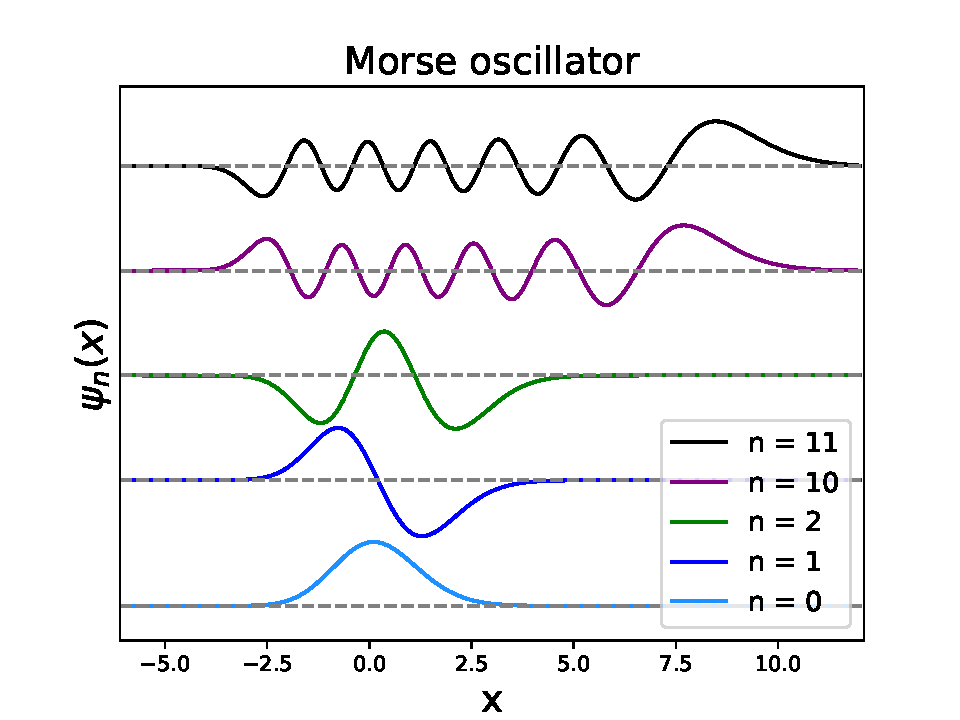
\includegraphics[width=40cm]{../plots/morse_states.pdf}
  \end{figure}
\end{block}

\begin{block}{Theory}
	Some Maths
\end{block}

\begin{block}{Methods}
	Some MeThOdS and Stuff
\end{block}

\begin{block}{References}
	Here is is
\end{block}

\end{column}
%==============================================================================%
% 			     	    Column 2				       %
%==============================================================================%
\begin{column}{0.50\linewidth}
\begin{block}{Methods}
Greetings
\end{block}

\begin{block}{Summary}
Hello
\end{block}

\end{column}
\end{columns}
\end{frame}
\end{document}
